\todo[inline]{Einleitung}

%%%%%%%%%%
\section{Architektur des Moodle-Plugins}
\label{sec:architektur}
Bei der Implementierung des Moodle-Plugins ist die durch Moodle vorgegebene Architektur von Plugins zu beachten \citep{moodle2016activity}. Diese besteht stets aus vorgegebenen Dateien und Ordnen, die Anzahl ist jeweils von der Art des zu entwickelnden Plugins abhängig. Darüber hinaus bestimmt die Art des Plugins auch den zu wählenden Speicherort.

Bei Activity Plugins, wie dem Plugin für Hyperaudio-Dokumente, ist als Speicherort der Ordner \textbf{/mod} vorgeben. In diesem Ordner muss ein Unterordner mit dem Namen des Plugins angelegt werden, in diesem Fall \textbf{hyperaudio}, in welchem alle Plugin-Dateien abgelegt werden. Eine Übersicht über die Ordnerstruktur des Hyperaudio-Plugins findet sich in Abbildung \ref{fig:Ordnerstruktur}.

\begin{figure}[h!]
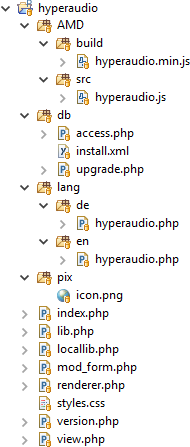
\includegraphics[width=0.3\textwidth,center]{Ordnerstruktur.PNG}
\caption{\label{fig:Ordnerstruktur}Ordnerstruktur des Hyperaudio-Plugins}
\end{figure}

Im Ordner \textbf{/hyperaudio/backup} werden die Dateien abgelegt, welche Anwendung finden, wenn ein Backup oder eine Wiederherstellung eines Kurses vorgenommen wird.

Der Ordner \textbf{/hyperaudio/db} beherbergt die Dateien \textbf{access.php}, \textbf{events.php}, \textbf{install.xml} und \textbf{upgrade.php}. Die Datei \textbf{access.php} dient zur Steuerung der Berechtigungen innerhalb des Moodle-Plugins, wobei den verschiedenen Moodle-Rollen verschiedene Rechte für die einzelnen Funktionen zugewiesen werden können. In der \textbf{events.php} können Beobachter eingerichtet werden, welche auf bestimmte Ereignisse warten. Bei der Installation des Plugins wird die \textbf{install.xml} zur Erstellung der Datenbanktabellen für das Plugin verwendet. Es ist mindestens eine Tabelle mit dem Namen des Plugins anzulegen. Sollten die Datenbanktabellen nach Veröffentlichung des Plugins um Spalten erweitert werden, so kommt die Datei \textbf{upgrade.php} zum Einsatz. Hierin werden die notwendigen Schritte für einen Versionsabgleich definiert.

Im Ordner \textbf{/hyperaudio/lang} wird die Sprachlokalisierung vorgenommen. Für jede Sprache wird innerhalb des \textbf{lang}-Ordners ein eigener Unterordner angelegt. Darin befindet sich jeweils eine PHP-Datei, in welcher die Übersetzungen definiert werden. Der Name dieser Datei entspricht wiederum dem Namen des Plugins.

Das Icon, welches für das Plugin  verwendet werden soll, muss im Ordner \textbf{/hyperaudio/pix} mit dem Dateinamen \textbf{icon.gif} abgelegt werden und sollte eine Auflösung von 16x16 Pixel besitzen.

Im Ordner \textbf{/hyperaudio} liegen dann die Dateien \textbf{lib.php}, \textbf{mod\underline{{ }}form.php}, \textbf{index.php}, \textbf{view.php} und \textbf{version.php}. Die \textbf{lib.php} dient dazu, Standardfunktionen von Moodle zu überschreiben, wobei \textit{add\underline{{ }}instance}, \textit{update\underline{{ }}instance} und \textit{delete\underline{{ }}instance} als essentielle Funktionen zu nennen sind. Mit diesen Funktionen wird das Anlegen, Aktualisieren und Löschen von Instanzen des Plugins ermöglicht. Zum Anlegen und Aktualisieren wird in der \textbf{mod\underline{{ }}form.php} die dazugehörige Maske festgelegt.


\textbf{\textit{index.php}}

\todo[inline]{index.php}

Die \textbf{view.php} ist die erste Datei, die beim Öffnen der Aktivität geladen wird und dient dementsprechend vornehmlich der Anzeige der Inhalte. In der \textbf{version.php} wird die Version des Plugins gepflegt. Erhöht sich die Versionsnummer in der \textbf{version.php}, wird der automatische Upgradeprozess von Moodle ausgelöst.

\todo[inline]{Ordnerstruktur aktualisieren}

%%%%%%%%%%
\section{Iterative Entwicklung}
Die Entwicklung des Plugins wird in iterativer Form durchgeführt. In jeder Iteration soll das Plugin nur um einige wenige Funktionalitäten erweitert werden. Jede Iteration soll mit einem lauffähigen Plugin abgeschlossen werden. So kann direkt das Ergebnis betrachtet werden und gegebenenfalls in der nächsten Iteration nochmals angepasst werden \citep{augsten2018iterativ}.

\subsection{Speichern und Abspielen einer Audio-Datei}
In der ersten Iteration wurde zunächst die grundlegende Struktur des Plugins erstellt (vgl. Abschnitt \ref{sec:architektur}). Hierbei wird in der Maske zum Anlegen und Aktualisieren von Instanzen des Hyperaudio-Plugins, neben dem obligatorischen Namens-Feld noch ein Element zum Hinzufügen einer Audiodatei angelegt. Hierfür wird der in Auflistung \ref{lst:it1:modform} dargestellt Code in der \textbf{mod\underline{{ }}form.php} ergänzt. Dieser Code wird in der Funktion \textit{public function definition()} der Klasse \textit{class mod\underline{{ }}hyperaudio\underline{{ }}mod\underline{{ }}form extends moodleform\underline{{ }}mod} verwendet. Der \textit{\underline{{ }}form} der \textit{moodleform\underline{{ }}mod} können neue Elemente hinzugefügt werden. Mit Hilfe von \textit{setType} und \textit{addRule} können den Elementen Typen und Bedingungen zugewiesen werden, im Fall von \textit{name} der Typ \textit{PARAM_TEXT} und die Bedingung \textit{required}. Bei Verwendung des Elements \textit{filemanager} können durch Verwendung eines Arrays Einschränkungen für Anzahl und Eigenschaften der hochzuladenden Dateien  festgelegt werden. \textit{get\underline{{ }}string} dient der Darstellung der lokalisierten Bezeichnung von Elementen.

\begin{lstlisting}[basicstyle=\small,
             inputencoding={utf8}, 
             extendedchars=false,
             commentstyle=\color{black}, 
             keywordstyle=\color{black}, 
             escapeinside=``,
             linewidth=\textwidth,
             caption={Ausschnitt der \textbf{mod\underline{{ }}form.php} in der 1. Iteration},
             label={lst:it1:modform}]
$mform = $this->_form;             
$mform->addElement(`'`text`'`, `'`name`'`, get_string(`'`hyperaudio_mod_form_name`'`, `'`hyperaudio`'`));
$mform->setType(`'`name`'`, PARAM_TEXT);
$mform->addRule(`'`name`'`, get_string(`'`error_wrong_hyperaudio_name_input`'`, `'`hyperaudio`'`), `'`required`'`);
$mform->addElement(`'`filemanager`'`, `'`audiofile`'`, get_string(`'`hyperaudiodata`'`, `'`hyperaudio`'`), null,
     array(
        `'`subdirs`'` => 0,
        `'`maxbytes`'` => 0,
		`'`areamaxbytes`'` => 10485760,
		`'`maxfiles`'` => 1,
		`'`accepted_types`'` => array(
			`'`audio`'`
		)
	)
);
$mform->addRule(`'`audiofile`'`, get_string(`'`required`'`, `'`hyperaudio`'`), `'`required`'`);
\end{lstlisting}

Neben der \textbf{mod\underline{{ }}form.php} muss auch die \textbf{lib.php} angepasste werden. Hierfür müssen die bereits beschriebenen Funktionen \textit{add\underline{{ }}instance}, \textit{update\underline{{ }}instance} und \textit{delete\underline{{ }}instance} erzeugt werden. Beispielhaft wird die Funktionen \textit{add\underline{{ }}instance} betrachtet. 

\begin{lstlisting}[basicstyle=\small,
             inputencoding={utf8}, 
             extendedchars=false,
             commentstyle=\color{black}, 
             keywordstyle=\color{black}, 
             escapeinside=``,
             linewidth=\textwidth,
             caption={Ausschnitt der \textbf{lib.php} in der 1. Iteration},
             label={lst:it1:lib}]
function hyperaudio_add_instance($data) {
    global $CFG, $DB;
    
    $cmid = $data->coursemodule;
    $context = context_module::instance($cmid);
    $draftitemid_audiofile = $data->audiofile;
    
    unset($data->audiofile);
     
    $now = time();
    $data->timecreated = $now;
    $data->timemodified = $now;
    
    $data->id = $DB->insert_record(`'`hyperaudio`'`, $data);
    
    hyperaudio_update_audiofile($data->id, $context, $draftitemid_audiofile);
     
    return $data->id;
}
\end{lstlisting}



\subsection{Speichern und Anzeige von Zusatzinhalten}
\dots

\subsection{Einbindung der Konfigurationsdatei}
\dots

\subsection{Speichern und Anzeige von Kommentaren}
\dots

\subsection{Antworten auf Kommentare}
\dots

\subsection{Galerie der Zusatzinhalte}
\dots

\subsection{Visualisierung der Annotationen in der Timeline}
\dots

%%%%%%%%%%
\section{Zusammenfassung}
\dots